\section{Results}

\subsection{Historical Operation of \gls{EU} Reactors}


\begin{table}[h]
	\centering
	\scalebox{0.86}{
		\begin{tabular}{|c|c|c|}
			\hline
			Category [unit] & Value & Specifics \\ \hline
			Total UOX Usage [t] & 188,196  &  \\ \hline
			Total MOX Usage [t] & 118 & \\ \hline
			Total Spent UOX [t] & 183,807 & \\ \hline
			Total Spent MOX [t] & 0 & All is Reprocessed. \\ \hline
			Total Tailings [t] & 1,127,905 & \\ \hline
			Total Natural U [t] & 1,316,959 & \\ \hline
		\end{tabular}}
		\caption{Simulation Results}
		\label{tab:sim_result}
		\end {table}

\Cref{tab:sim_result} lists the important metrics
obtained from the first simulation. The following
values are the \gls{EU} inventory and history at year 2050.

Figures \ref{fig:eu_num} and \ref{fig:eu_pow} display the
timeseries of number of reactors and installed capacity in \gls{EU}.


\begin{figure}[htbp!]
	\begin{center}
		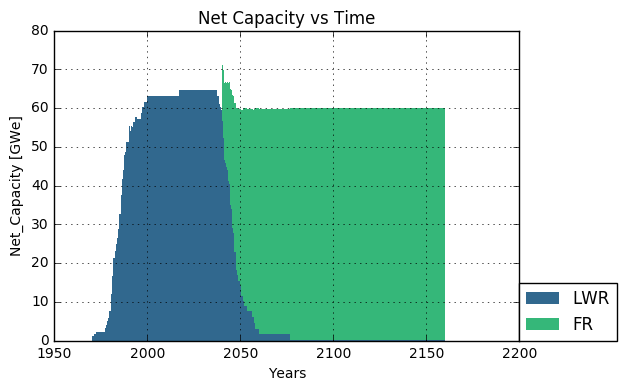
\includegraphics[scale=0.7]{./images/eu_future/number_plot.png}
	\end{center}
	\caption{Timeseries of number of reactors in \gls{EU}.}
	\label{fig:eu_num}
\end{figure}

\begin{figure}[htbp!]
	\begin{center}
		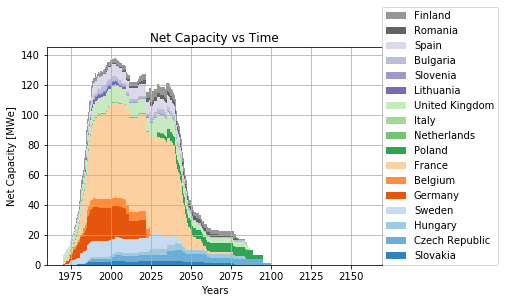
\includegraphics[scale=0.7]{./images/eu_future/power_plot.png}
	\end{center}
	\caption{Timeseries of installed nuclear capacity in \gls{EU}.}
	\label{fig:eu_pow}
\end{figure}
\FloatBarrier


Figures \ref{fig:eu_tail} and \ref{fig:eu_snf} show the 
timeseries of mass of tailings and spent fuel accumulation in \gls{EU}.

Figure \ref{fig:eu_fuel} shows the amount of fuel used in \gls{EU}.


\begin{figure}[htbp!]
	\begin{center}
		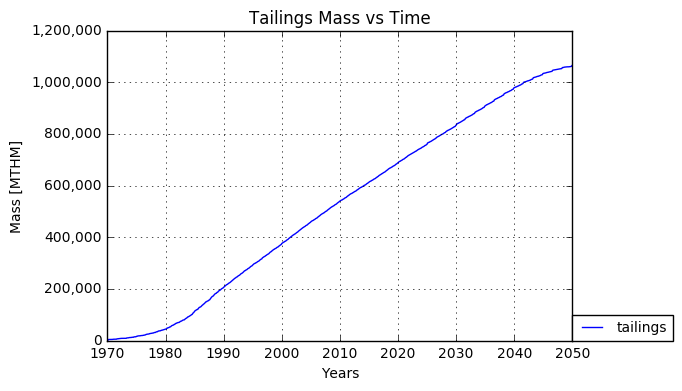
\includegraphics[scale=0.7]{./images/eu_future/tailings.png}
	\end{center}
	\caption{Timeseries of Tailings in the \gls{EU}.}
	\label{fig:eu_tail}
\end{figure}

\begin{figure}[htbp!]
	\begin{center}
		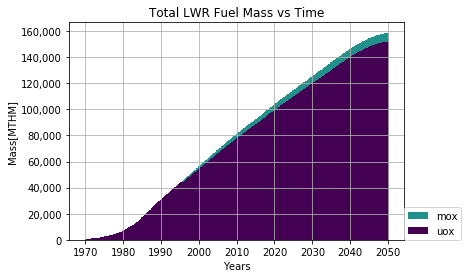
\includegraphics[scale=0.7]{./images/eu_future/total_fuel.png}
	\end{center}
	\caption{Timeseries of total fuel usage in \gls{EU}.}
	\label{fig:eu_fuel}
\end{figure}


\begin{figure}[htbp!]
	\begin{center}
			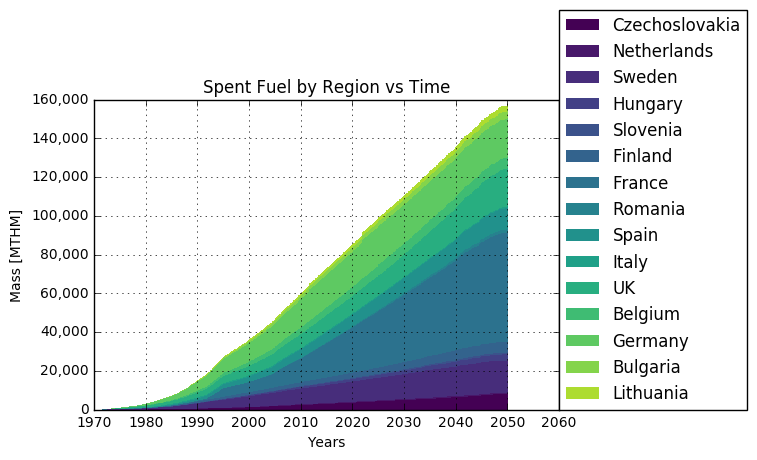
\includegraphics[scale=0.7]{./images/eu_future/snf.png}
	\end{center}
	\caption{Timeseries of Spent Nuclear Fuel.}
	\label{fig:eu_snf}
\end{figure}
\FloatBarrier

Note that the MOX usage is so little that it is invisible in the
plot. 

\begin{table}[h]
	\centering
	\begin{tabular}{|c|c|c|}
		\hline
		Isotope & Mass Fraction in Spent Fuel [\%] & Quantity [t] \\ \hline
		Total & .9358 & 1,720 \\ \hline
		Pu238 & .0111 & 20.40 \\ \hline
		Pu239 & .518 & 952.12 \\ \hline
		Pu240 & .232 & 426.43 \\ \hline
		Pu241 & .126 & 231.59 \\ \hline
		Pu242 & .0487 & 89.51 \\ \hline
	\end{tabular}
	\caption{Plutonium From Spent Fuel}
	\label{tab:pu}
\end{table}


To create \gls{MOX}, 9\% Pu and 91\% depleted uranium is used.
Thus $1,720$ tons of plutonium yields $19,111$ tons of
\gls{MOX}. \Cref{tab:pu} lists the isotope, mass fraction,
and quantity of plutonium that can be obtained from the 2050 \gls{SNF} inventory.


\subsection{French \gls{SFR} Transition Scenario}

From Varaine et al. \cite{marsaultmarie-sophie_pre-conceptual_2012}, a French
ASTRID-type \gls{SFR} of capacity 600 MWe needs $1.225$ tons of
plutonium a year, with an initial plutonium loading of $4.9$ tons. 
Thus, the number of \glspl{SFR} that can be loaded with the reprocessed
plutonium from \gls{SNF} can be estimated to $\frac{1,720}{4.9} \approx 351$ \glspl{SFR},
assuming infinite reprocessing and fabrication capacity as well as
abundant depleted uranium supply. 

Also, assuming that \gls{MOX} can be recycled indefinitely,
spent \gls{MOX} from an ASTRID reactor
contains enough plutonium to produce a \gls{MOX} fuel with
the same mass, if mixed with depleted uranium. For example,
spent \gls{MOX} from an ASTRID reactor is 12.6\% plutonium,
whereas a fresh \gls{MOX} is 9\% plutonium.
The compositions are in \cref{tab:comp}.
Separating plutonium from spent \gls{MOX} from
an ASTRID reactor can create \gls{MOX} of the mass of spent \gls{MOX}.

The second scenario, with the tails and spent \gls{UOX}
inventory, evaluates if the French can transition into \gls{SFR}
without constructing additional \gls{LWR}s. This simulation
assumed infinite reprocessing and fabrication capacity.

\Cref{fig:fuel} shows the mass of \gls{MOX} used in the 
\gls{SFR}s separated by how they are made, over time.
Note that the mass of \gls{MOX} from the spent \gls{UOX}
stops increasing around 2050, which means that the spent
\gls{MOX} is enough to create the \gls{MOX} for the
\gls{SFR} fleet. 

\begin{figure}[htbp!]
	\begin{center}
		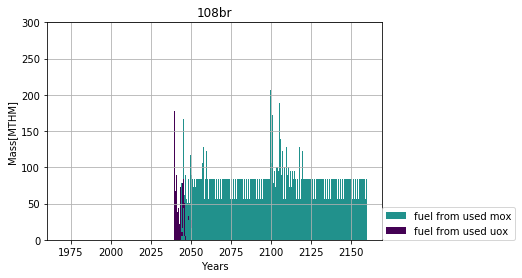
\includegraphics[scale=0.7]{./images/french-transition/where_fuel.png}
	\end{center}
	\caption{Timeseries of fuel used in the \gls{SFR}s [tons]}
	\label{fig:fuel}
\end{figure}

\Cref{fig:pu_demand} shows the separated plutonium demand
 from spent \gls{MOX} to fuel the ASTRID reactors.

\Cref{fig:reprocess_waste} shows the amount of reprocessing waste
(any content from spent fuel other than U, Pu) over time. Note that 
the amount of reprocessing waste is much greater when reprocessing
spent \gls{MOX} from ASTRID reactors, since there is little uranium
or plutonium left due to a high burnup.

\Cref{fig:pu_isotopics} shows the isotopics of the plutonium that are
reprocessed from the spent fuel inventory. Note the increase in 2040 is due to
ASTRID reactors produce high plutonium spent fuel.

\begin{figure}[htbp!]
	\begin{center}
		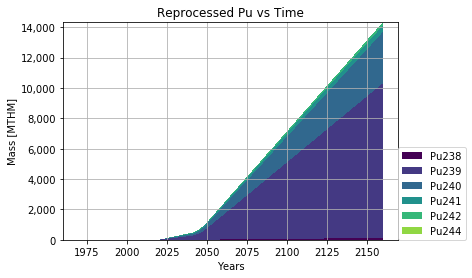
\includegraphics[scale=0.7]{./images/french-transition/rep_pu.png}
	\end{center}
	\caption{Plutonium timeseries separated by isotope}
	\label{fig:pu_isotopics}
\end{figure}

\begin{figure}[htbp!]
	\begin{center}
		\includegraphics[scale=0.7]{./images/french-transition/pu_demand.png}
	\end{center}
	\caption{Separated Plutonium demand from Spent MOX}
	\label{fig:pu_demand_mox}
\end{figure}

\begin{figure}[htbp!]
	\begin{center}
		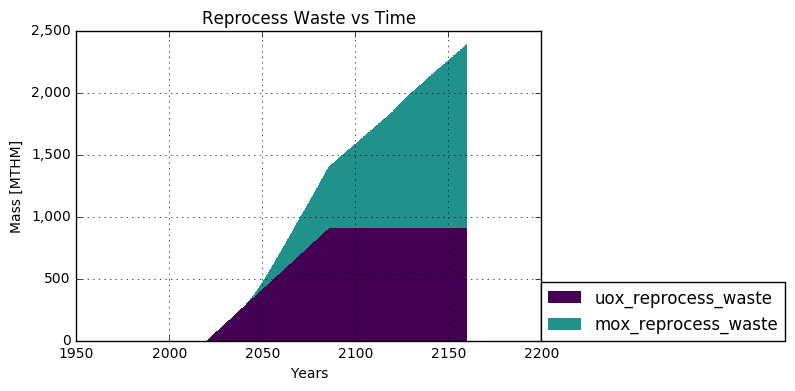
\includegraphics[scale=0.7]{./images/french-transition/reprocess_waste.png}
	\end{center}
	\caption{Reprocessing Waste for French Transition Scenario.}
	\label{fig:reprocess_waste}
\end{figure}


\begin{table}[h]
	\centering
	\scalebox{0.86}{
		\begin{tabular}{|c|c|}
			\hline
			Category [unit] & Value  \\ \hline
			Total MOX used [t] & 169,960  \\ \hline
			Total Reactors Deployed & 200 \\ \hline
			Total MOX from UOX Waste [t] & 19,136  \\ \hline
			Total MOX from MOX Waste [t] & 150,823  \\ \hline
			Total Tailings used [t] & 154,663  \\ \hline
			Total legacy SNF reprocessed [t] & 183,688 \\ \hline
		\end{tabular}}
		\caption {\gls{SFR} Simulation Results}
		\label{tab:sfr_sim_result}
\end {table}


